\documentclass{article}

\usepackage{subcaption}
\usepackage[labelformat=parens,labelsep=quad,skip=3pt]{caption}
\usepackage{graphicx}
\usepackage{geometry}

%\geometry{top=0.1in, left=0.1in, right=0.1in, bottom=0.1in}

\usepackage{array}
\usepackage{makecell}
\usepackage{tabularx}
\usepackage[dvipsnames]{xcolor}
\usepackage{amssymb}
\renewcommand{\tabularxcolumn}[1]{m{#1}}

%\pdfpageheight=5in
%\pdfpagewidth=7.2in

\begin{document}
	\section{Single-subject Results}
	\begin{figure}
		\begin{tabularx}{\textwidth}{|X|X|}
			\multicolumn{1}{c}{\textbf{Classical GLM}} & \multicolumn{1}{c}{\textbf{Bayesian GLM}}  \\ \hline
			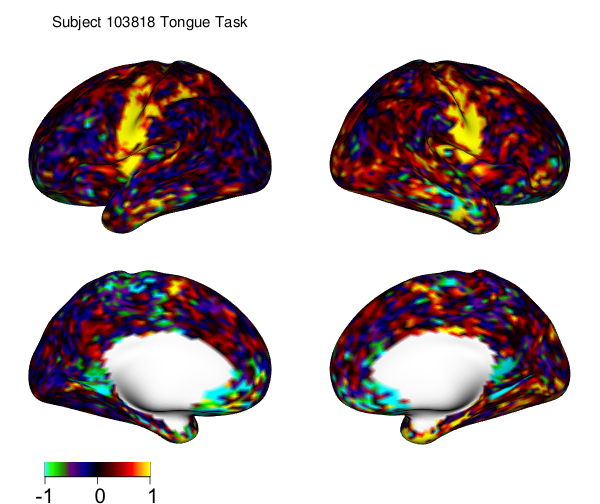
\includegraphics[width=0.48\textwidth]{plots/600_subject_103818_tongue_classical_estimates.png} &
			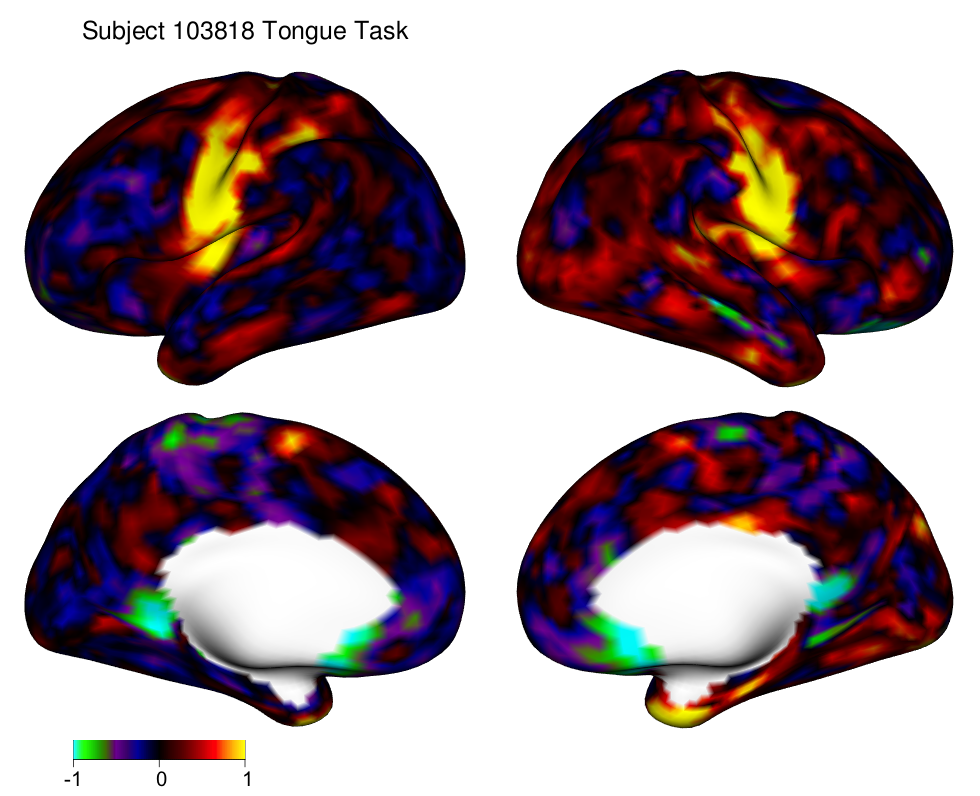
\includegraphics[width=0.48\textwidth]{plots/600_subject_103818_tongue_estimates.png} \\ \hline
			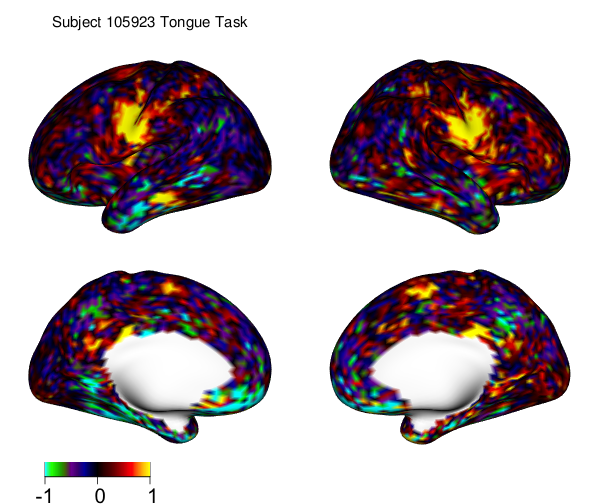
\includegraphics[width=0.48\textwidth]{plots/600_subject_105923_tongue_classical_estimates.png} &
			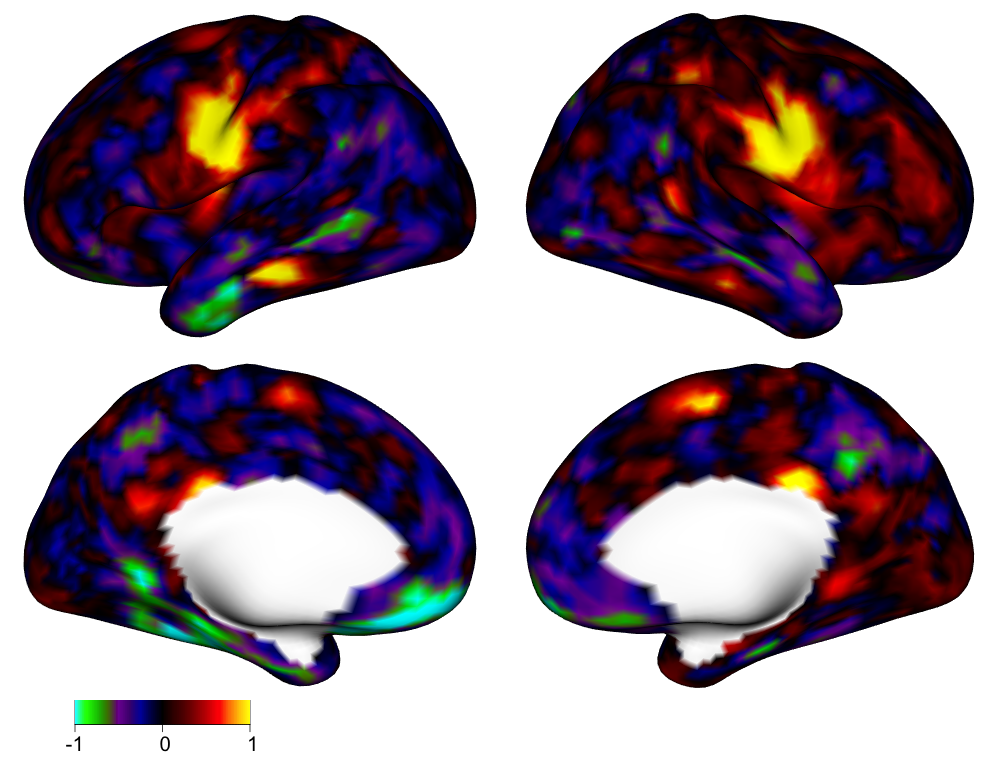
\includegraphics[width=0.48\textwidth]{plots/600_subject_105923_tongue_estimates.png} \\ \hline
			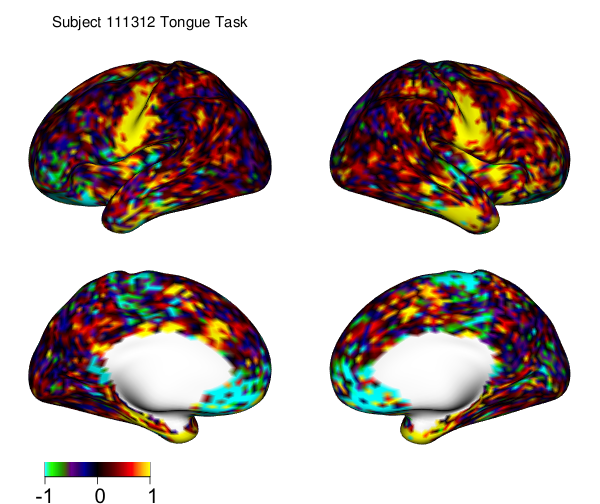
\includegraphics[width=0.48\textwidth]{plots/600_subject_111312_tongue_classical_estimates.png} &
			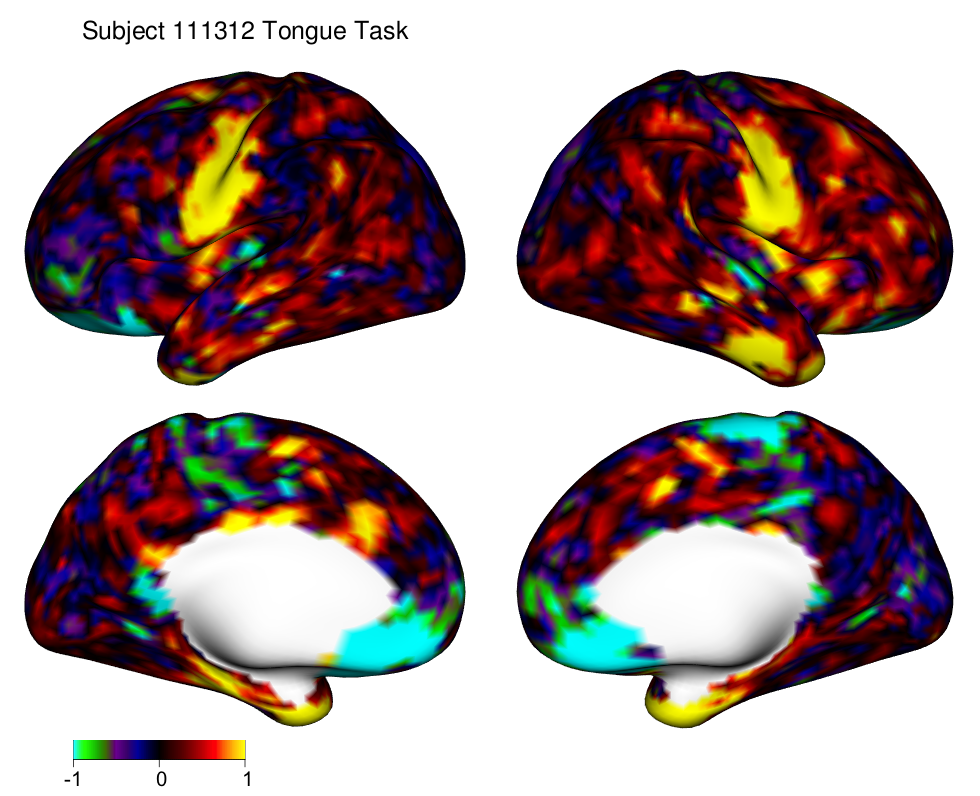
\includegraphics[width=0.48\textwidth]{plots/600_subject_111312_tongue_estimates.png} \\ \hline
			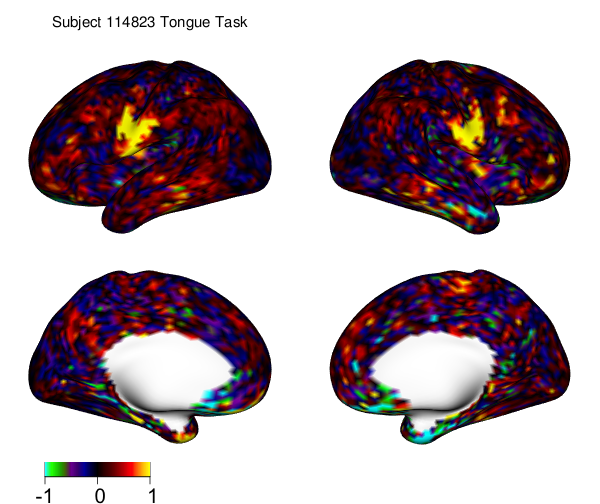
\includegraphics[width=0.48\textwidth]{plots/600_subject_114823_tongue_classical_estimates.png} &
			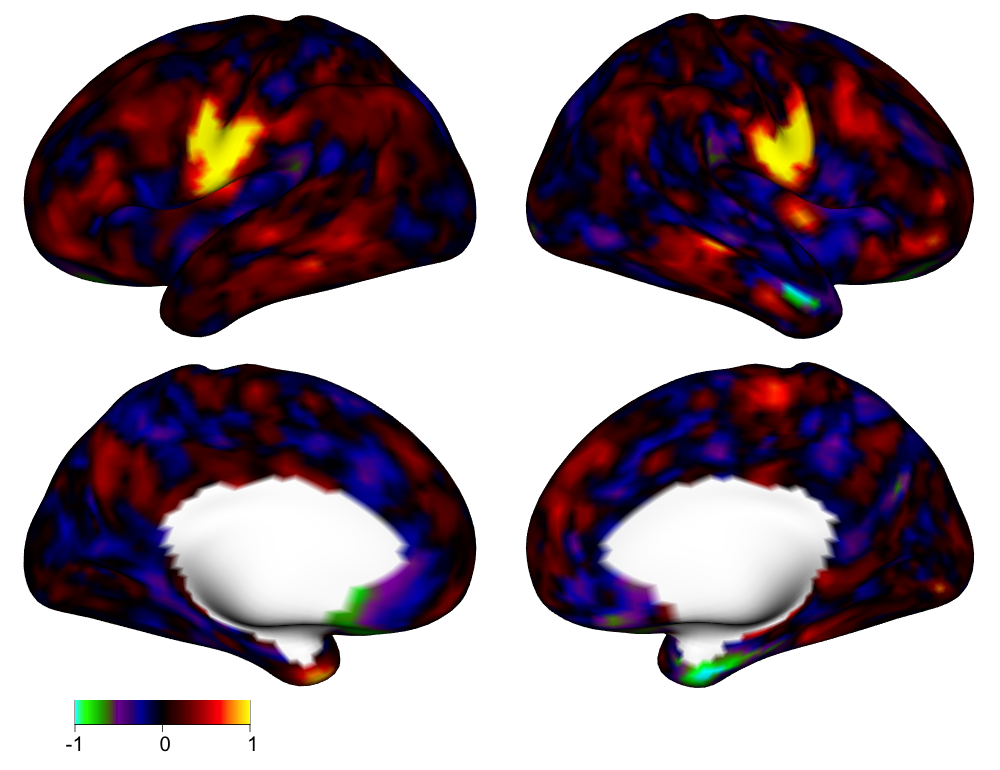
\includegraphics[width=0.48\textwidth]{plots/600_subject_114823_tongue_estimates.png} \\ \hline
%			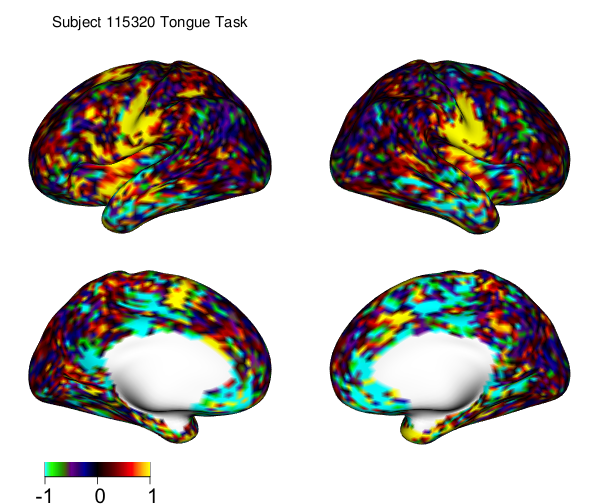
\includegraphics[width=0.48\textwidth]{plots/600_subject_115320_tongue_classical_estimates.png} &
%			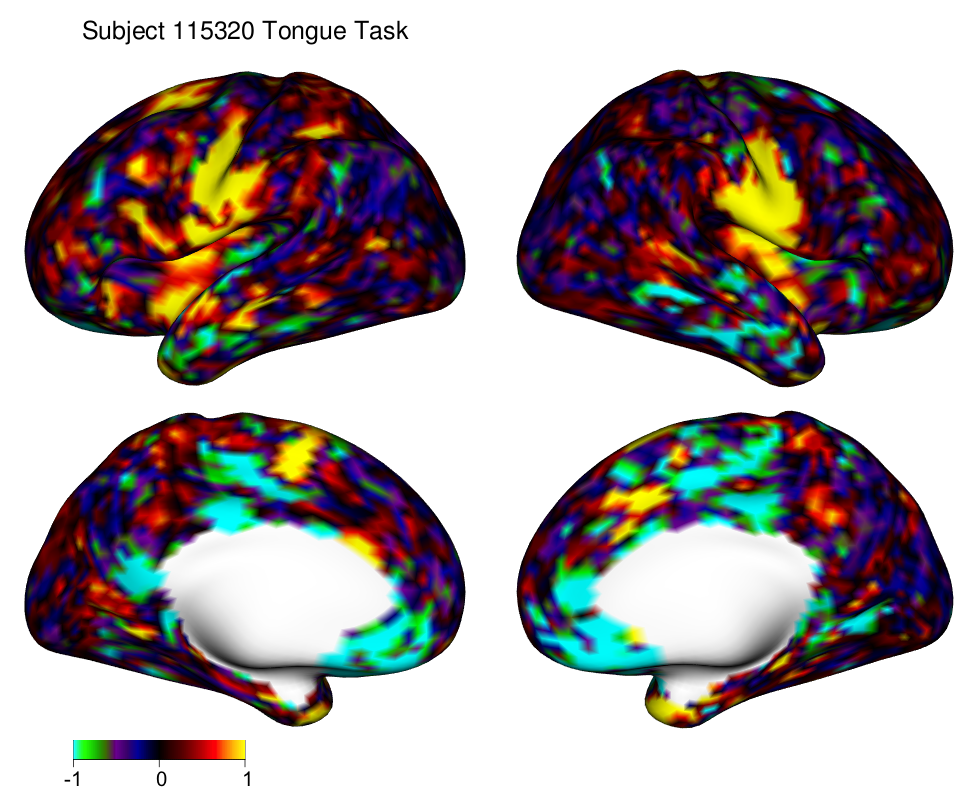
\includegraphics[width=0.48\textwidth]{plots/600_subject_115320_tongue_estimates.png} \\ \hline
		\end{tabularx}
		\caption{Single-subject estimates of activation amplitude for both brain hemispheres for the tongue task.}
		\label{fig:tongue_est_single_subject}
	\end{figure}

	\begin{figure}
		\begin{tabularx}{\textwidth}{|X|X|}
			\multicolumn{1}{c}{\textbf{Classical GLM}} & \multicolumn{1}{c}{\textbf{Bayesian GLM}}  \\ \hline
			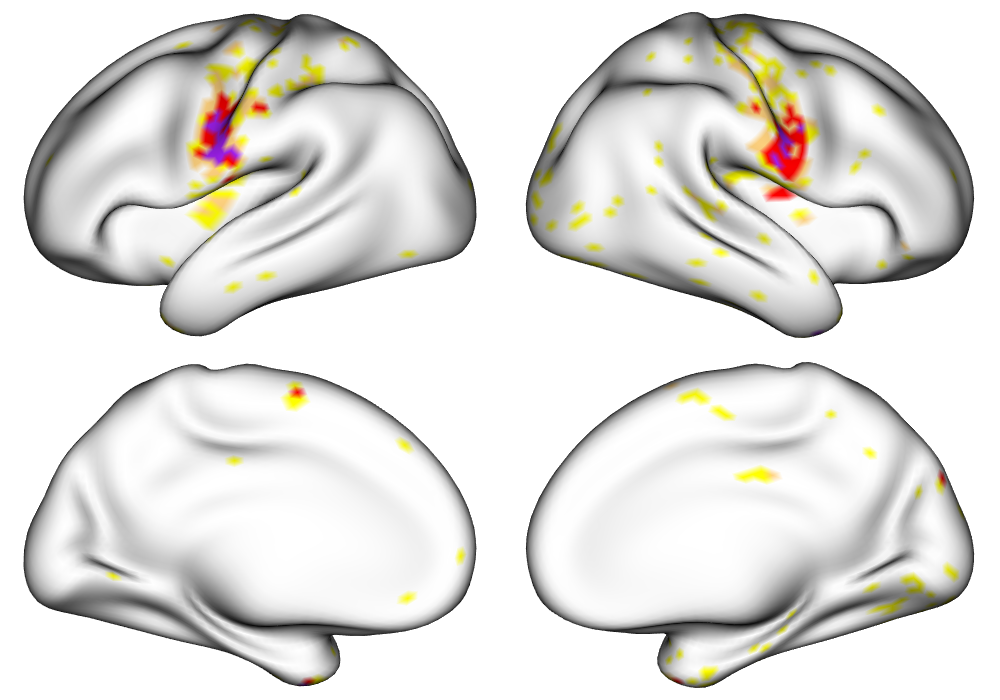
\includegraphics[width=0.48\textwidth]{plots/603_subject_103818_tongue_task_activations_classical.png} &
			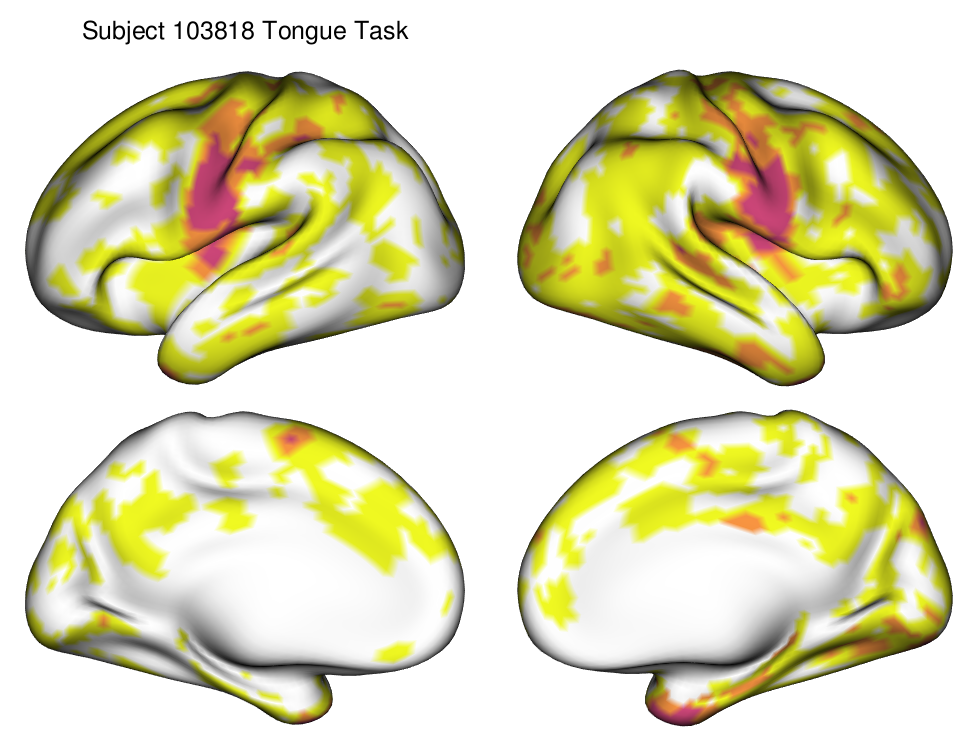
\includegraphics[width=0.48\textwidth]{plots/603_subject_103818_tongue_task_activations.png} \\ \hline
			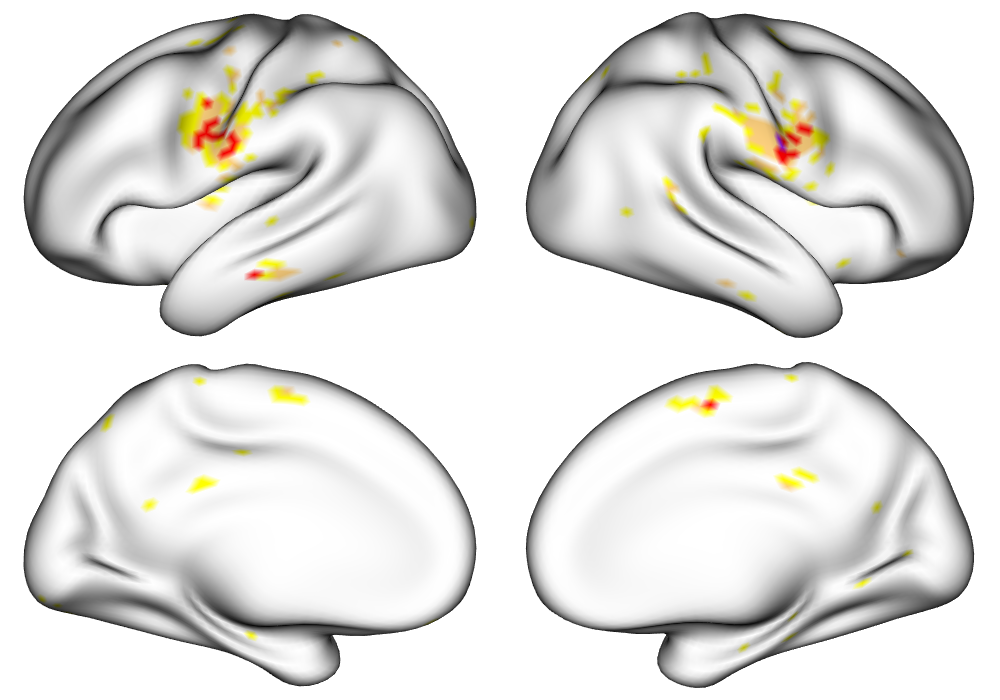
\includegraphics[width=0.48\textwidth]{plots/603_subject_105923_tongue_task_activations_classical.png} &
			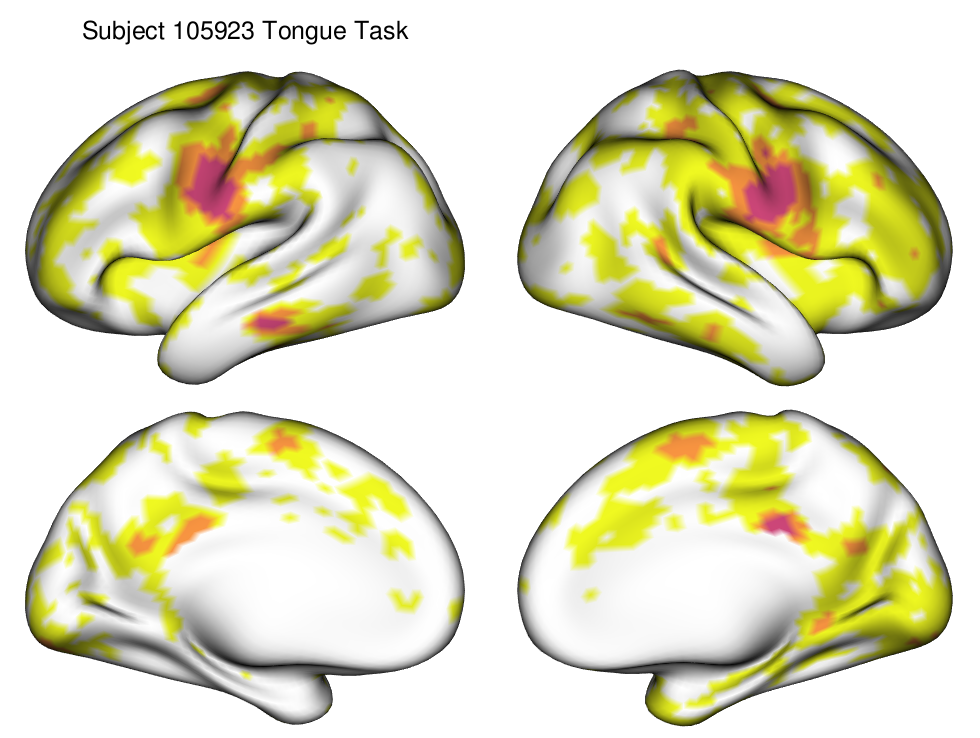
\includegraphics[width=0.48\textwidth]{plots/603_subject_105923_tongue_task_activations.png} \\ \hline
%			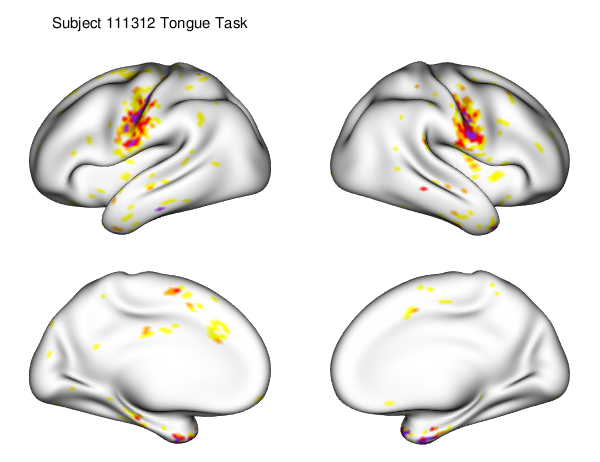
\includegraphics[width=0.48\textwidth]{plots/603_subject_111312_tongue_task_activations_classical.png} &
%			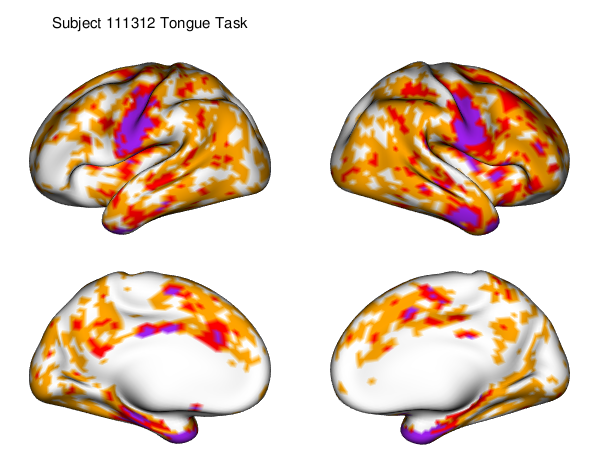
\includegraphics[width=0.48\textwidth]{plots/603_subject_111312_tongue_task_activations.png} \\ \hline
			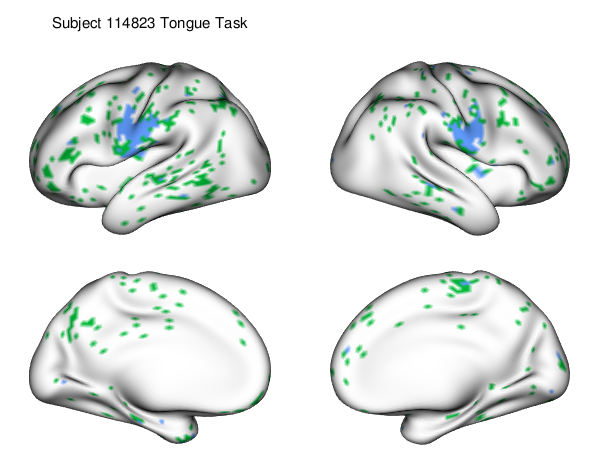
\includegraphics[width=0.48\textwidth]{plots/603_subject_114823_tongue_task_activations_classical.png} &
			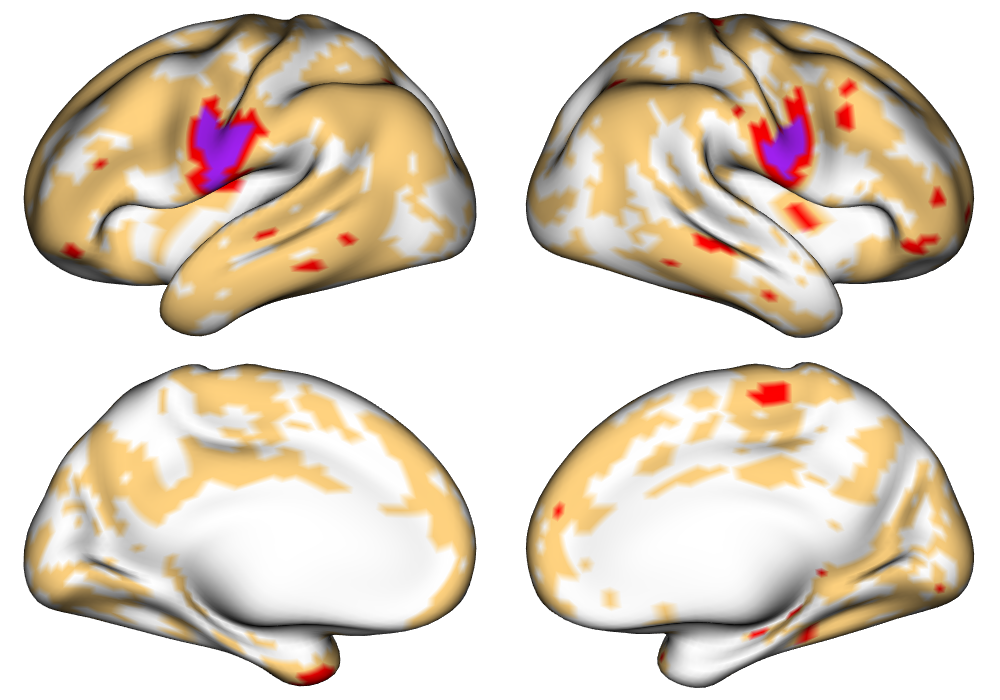
\includegraphics[width=0.48\textwidth]{plots/603_subject_114823_tongue_task_activations.png} \\ \hline
%			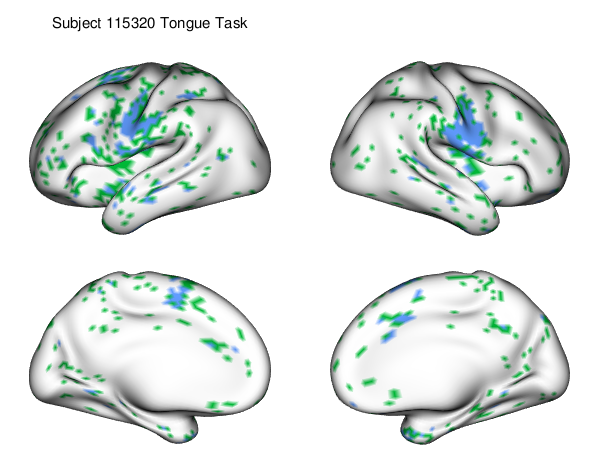
\includegraphics[width=0.48\textwidth]{plots/603_subject_115320_tongue_task_activations_classical.png} &
%			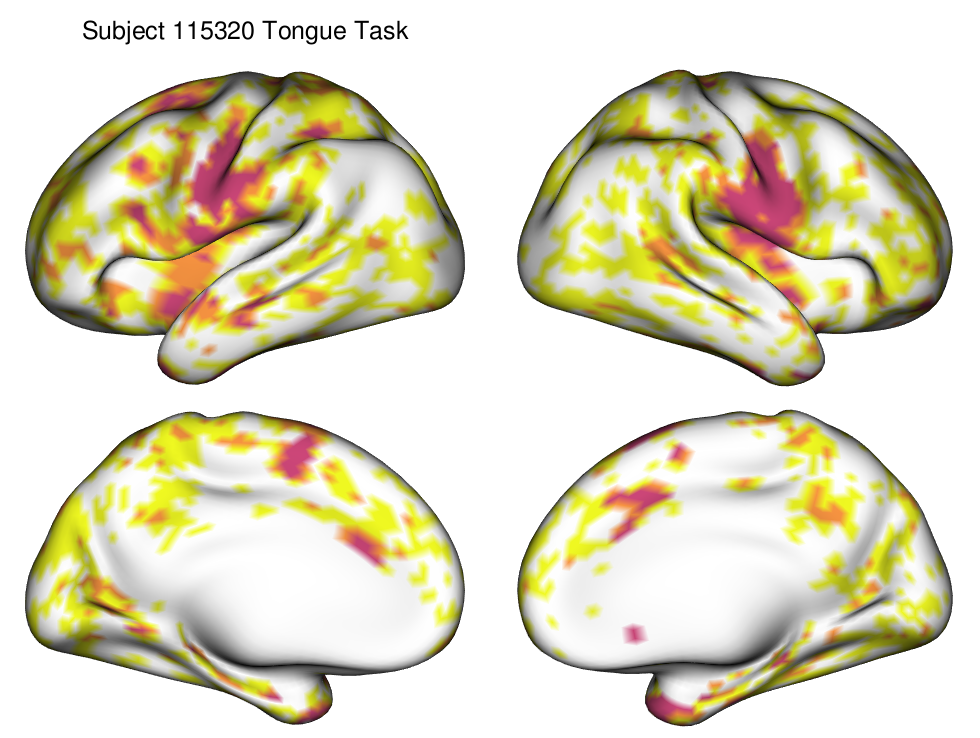
\includegraphics[width=0.48\textwidth]{plots/603_subject_115320_tongue_task_activations.png} \\ \hline
		\end{tabularx}
		\caption{Single-subject activations for both brain hemispheres for the tongue task.}
		\label{fig:tongue_act_single_subject}
	\end{figure}

\begin{figure}
	\begin{tabularx}{\textwidth}{|X|X|}
		\multicolumn{1}{c}{\textbf{Classical GLM}} & \multicolumn{1}{c}{\textbf{Bayesian GLM}}  \\ \hline
		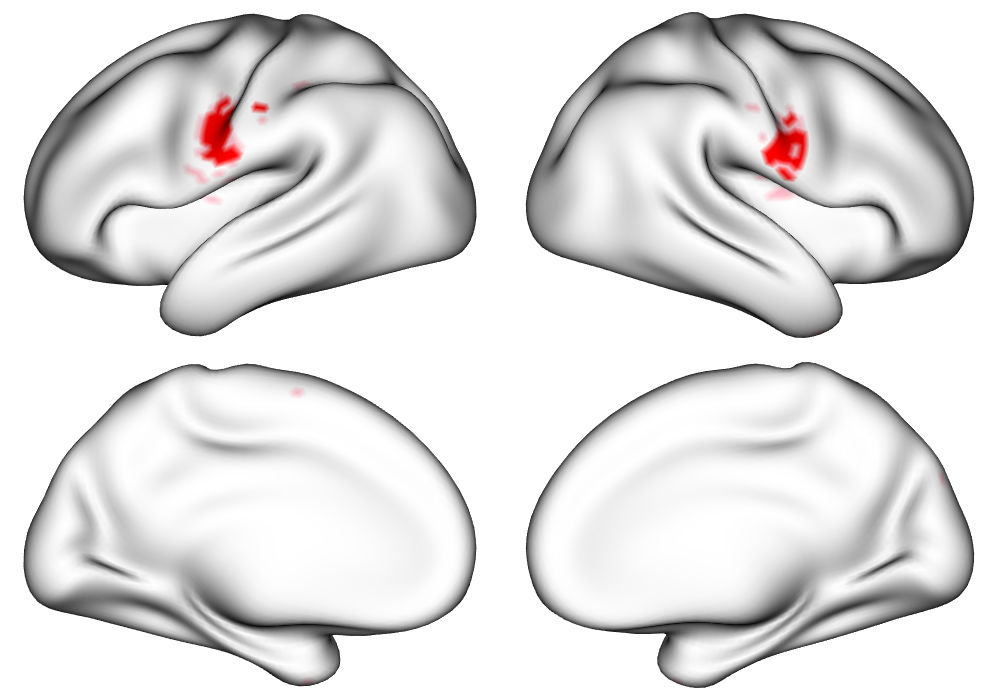
\includegraphics[width=0.48\textwidth]{plots/603_subject_103818_thr05_alpha001_num_active_classical.png} &
		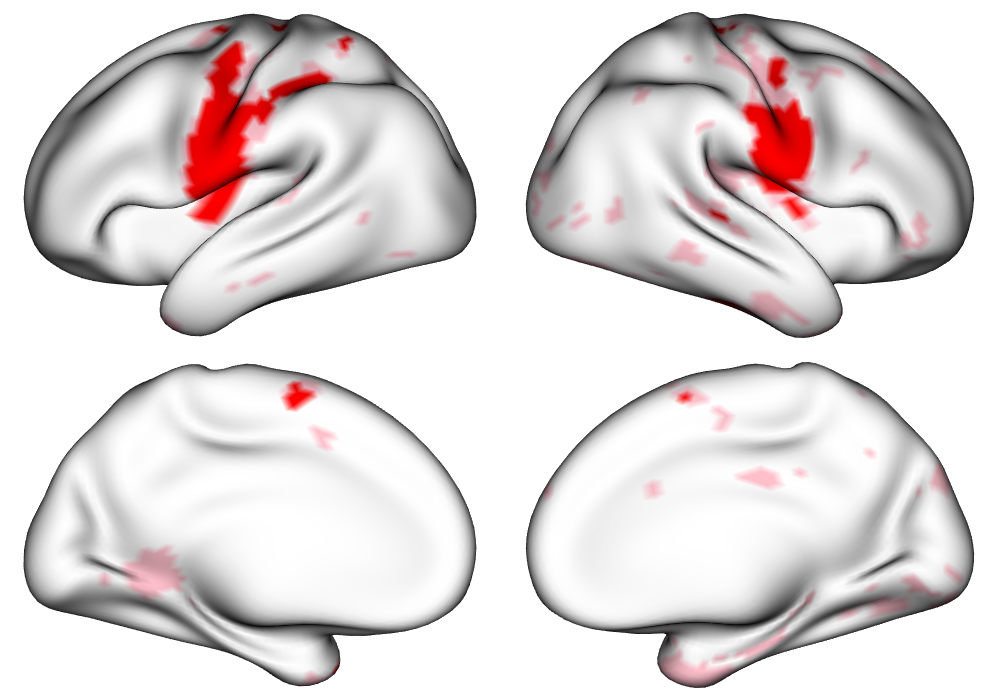
\includegraphics[width=0.48\textwidth]{plots/603_subject_103818_thr05_alpha001_num_active.png} \\ \hline
		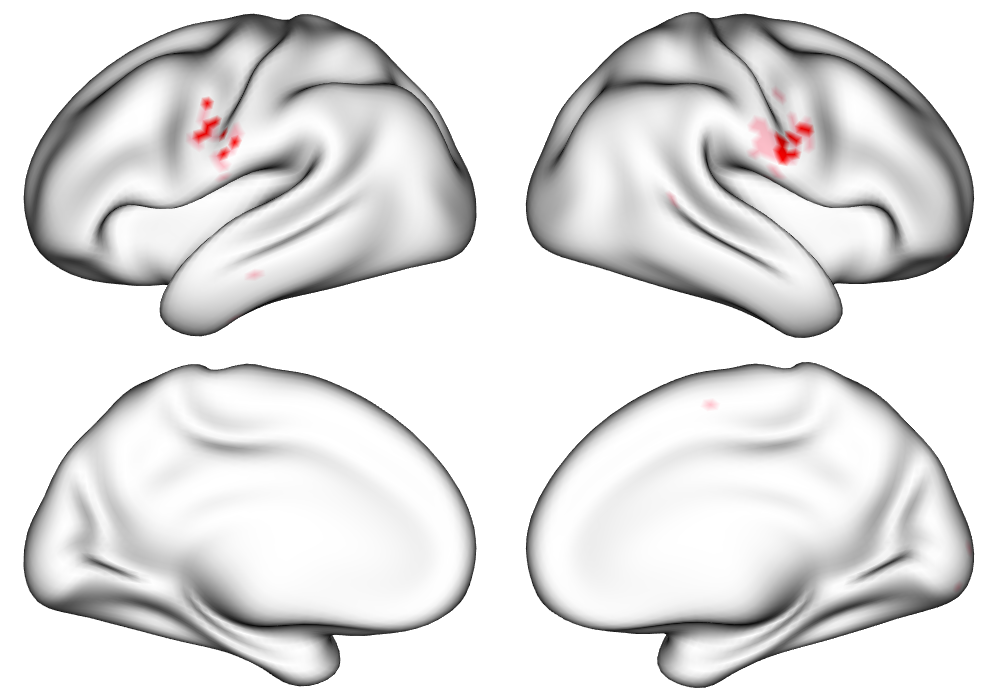
\includegraphics[width=0.48\textwidth]{plots/603_subject_105923_thr05_alpha001_num_active_classical.png} &
		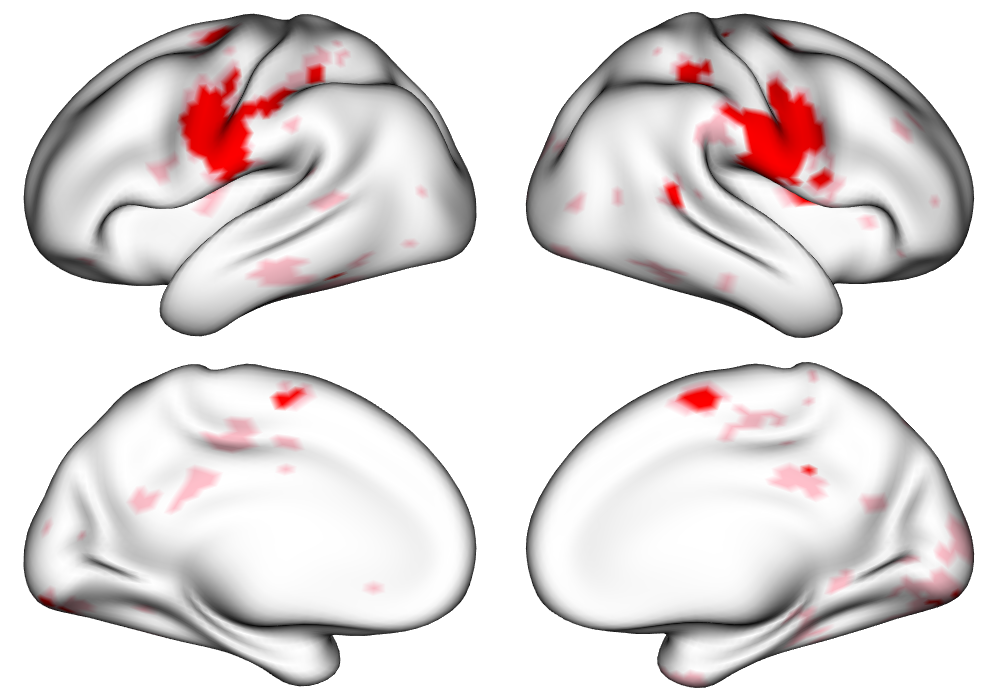
\includegraphics[width=0.48\textwidth]{plots/603_subject_105923_thr05_alpha001_num_active.png} \\ \hline
		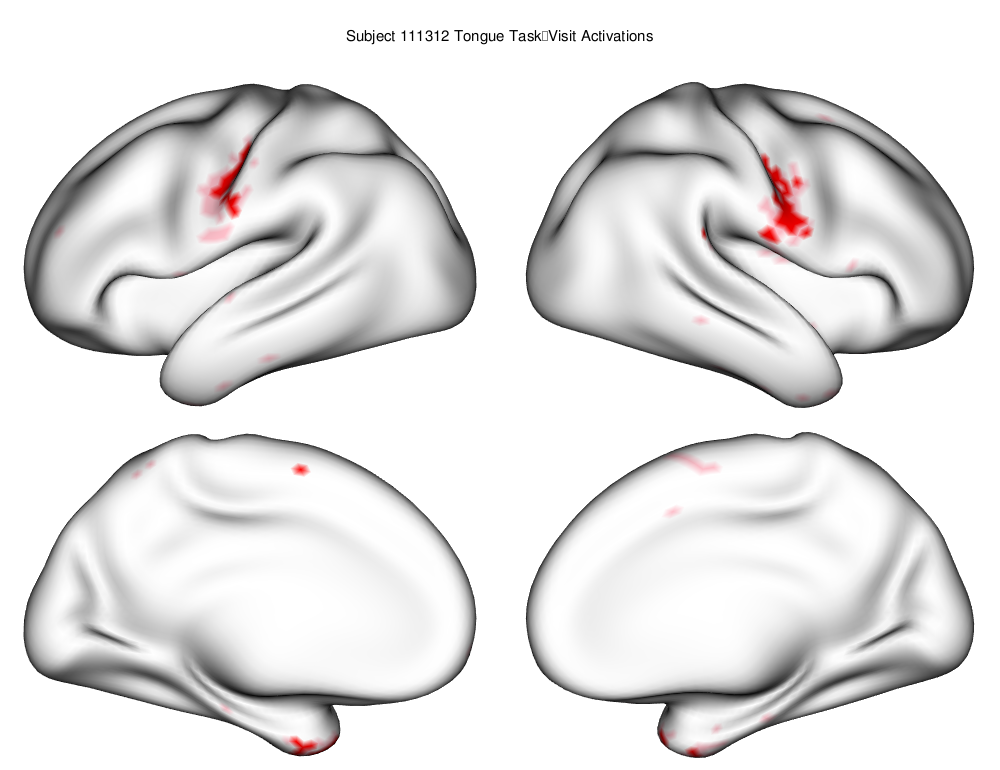
\includegraphics[width=0.48\textwidth]{plots/603_subject_111312_thr05_alpha001_num_active_classical.png} &
		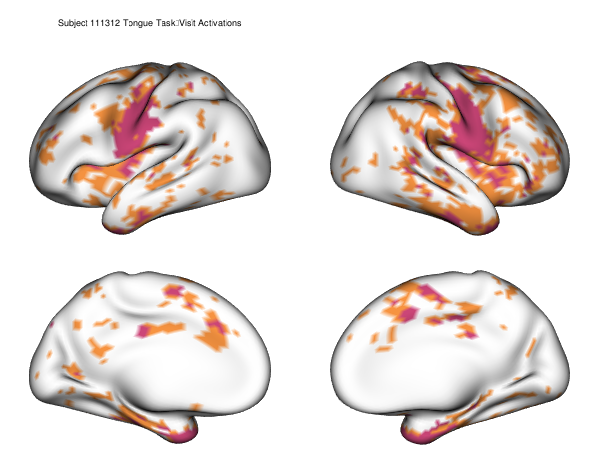
\includegraphics[width=0.48\textwidth]{plots/603_subject_111312_thr05_alpha001_num_active.png} \\ \hline
		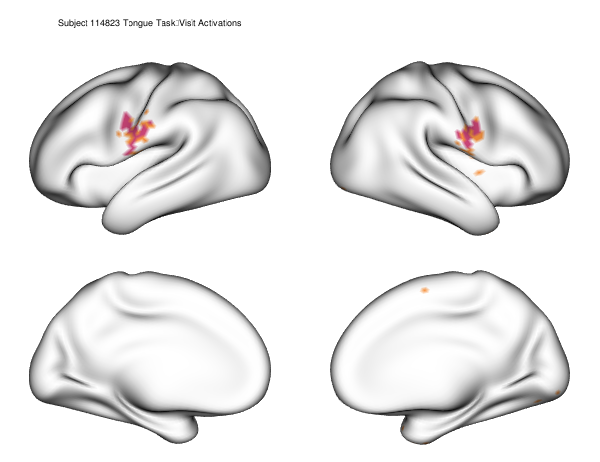
\includegraphics[width=0.48\textwidth]{plots/603_subject_114823_thr05_alpha001_num_active_classical.png} &
		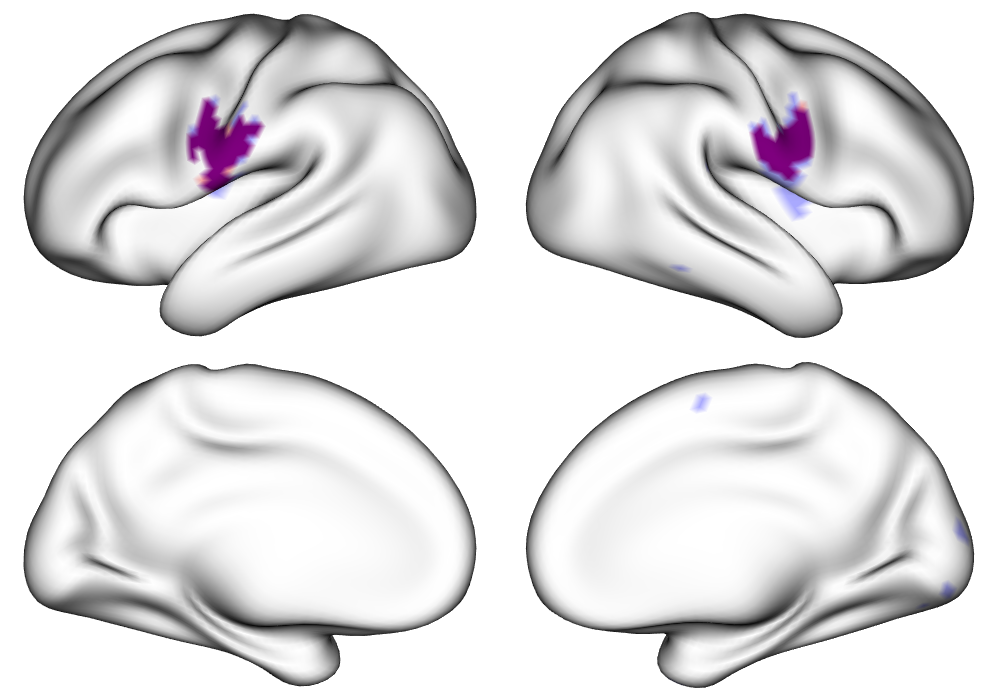
\includegraphics[width=0.48\textwidth]{plots/603_subject_114823_thr05_alpha001_num_active.png} \\ \hline
		%			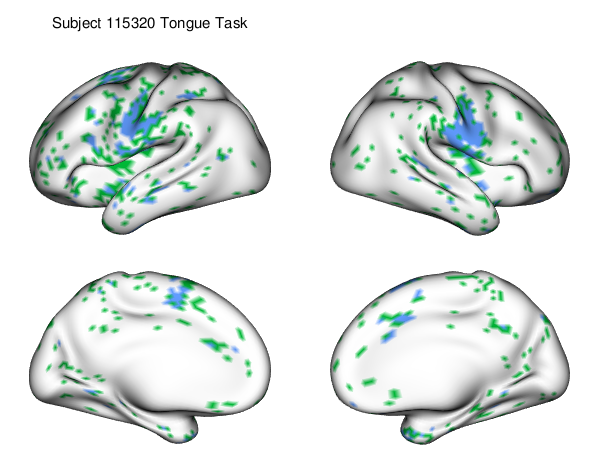
\includegraphics[width=0.48\textwidth]{plots/603_subject_115320_tongue_task_activations_classical.png} &
		%			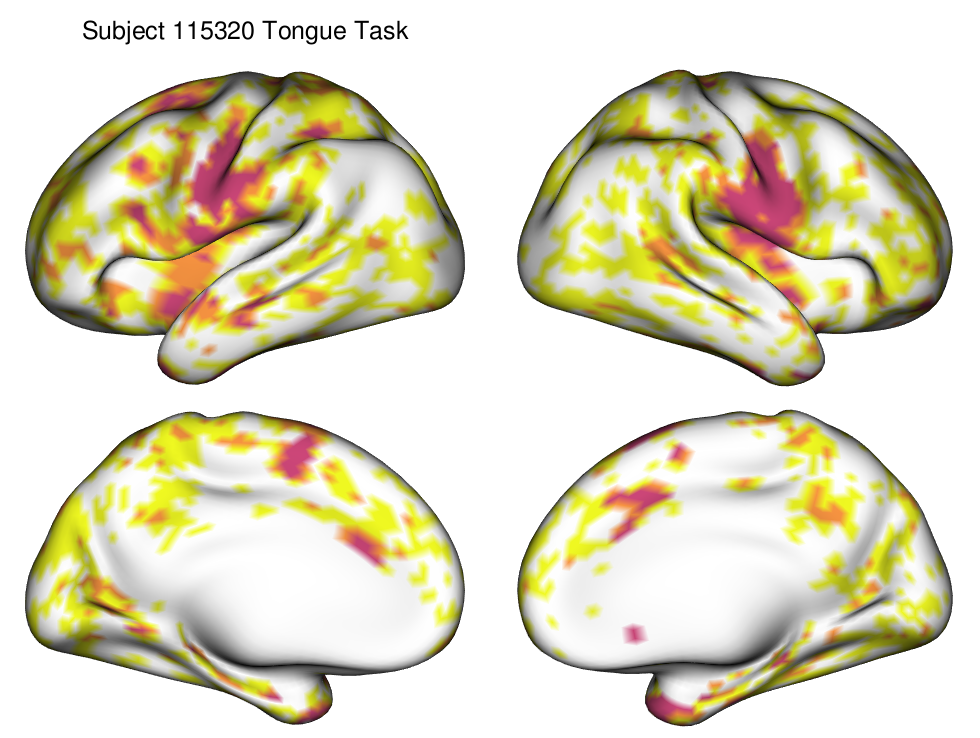
\includegraphics[width=0.48\textwidth]{plots/603_subject_115320_tongue_task_activations.png} \\ \hline
	\end{tabularx}
	\caption{Number of detected activations across the two visits for the tongue task at $\gamma=0.5\%$ and $\alpha = 0.01$.}
	\label{fig:tongue_act_single_subject_two_visits}
\end{figure}
	
\end{document}